% ===============================================================
% APRESENTAÇÃO PRÉVIA (ACOMPANHAMENTO) - TCC2 - SENAC SANTO AMARO
% ===============================================================
% Baseada em apresentacao_tcc2.tex (template do curso).
% Compilar a partir da pasta tcc2/:
%   pdflatex apresentacao_previa.tex   (2x)
% ===============================================================

\documentclass[
    aspectratio=169,
    12pt,
    brazil
]{beamer}

% ---------------------------------------------------------------
% PACOTES
% ---------------------------------------------------------------
\usepackage[T1]{fontenc}
\usepackage[utf8]{inputenc}
\usepackage[brazil]{babel}
\usepackage{graphicx}
\usepackage{booktabs}
\usepackage{array}
\usepackage{tikz}
\usetikzlibrary{arrows.meta,positioning,fit,calc}
\usepackage{pgfplots}
\pgfplotsset{compat=1.18}
\usepgfplotslibrary{groupplots}
\usepackage{appendixnumberbeamer}

% ---------------------------------------------------------------
% TEMA E CORES (template do curso)
% ---------------------------------------------------------------
\usetheme{default}
\useinnertheme{circles}
\setbeamertemplate{navigation symbols}{}

\definecolor{senacblue}{RGB}{0,51,102}
\definecolor{senacorange}{RGB}{243,146,0}

\setbeamercolor{structure}{fg=senacblue}
\setbeamercolor{frametitle}{fg=white,bg=senacblue}
\setbeamercolor{title}{fg=senacblue}
\setbeamercolor{section in toc}{fg=senacblue}
\setbeamercolor{itemize item}{fg=senacorange}
\setbeamercolor{itemize subitem}{fg=senacorange}
\setbeamerfont{frametitle}{series=\bfseries}
\setbeamertemplate{frametitle}[default][left]

\setbeamertemplate{footline}{%
  \leavevmode%
  \hbox{%
    \begin{beamercolorbox}[wd=.34\paperwidth,ht=2.4ex,dp=1ex,leftskip=1em]{author in head/foot}%
      \usebeamerfont{author in head/foot}\insertshortauthor
    \end{beamercolorbox}%
    \begin{beamercolorbox}[wd=.5\paperwidth,ht=2.4ex,dp=1ex,center]{title in head/foot}%
      \usebeamerfont{title in head/foot}\insertshorttitle
    \end{beamercolorbox}%
    \begin{beamercolorbox}[wd=.16\paperwidth,ht=2.4ex,dp=1ex,rightskip=1em]{title in head/foot}%
      \usebeamerfont{title in head/foot}\hfill\insertframenumber/\inserttotalframenumber
    \end{beamercolorbox}%
  }\vskip0pt%
}
\setbeamercolor{author in head/foot}{bg=senacblue,fg=white}
\setbeamercolor{title in head/foot}{bg=senacblue!85,fg=white}

% ---------------------------------------------------------------
% LOGO DO SENAC
% ---------------------------------------------------------------
\newcommand{\logosenacgrande}{%
  \IfFileExists{assets/logo-senac.png}{%
    
\includegraphics[height=2.2cm]{assets/logo-senac.png}%
  }{\fbox{\bfseries\color{senacblue}SENAC}}%
}
\newcommand{\logosenacpequena}{%
  \IfFileExists{assets/logo-senac.png}{%
    
\includegraphics[height=0.8cm]{assets/logo-senac.png}%
  }{\fbox{\scriptsize\bfseries\color{senacblue}SENAC}}%
}
\addtobeamertemplate{frametitle}{}{%
  \begin{tikzpicture}[remember picture,overlay]
    \node[anchor=north east,fill=white,rounded corners=2pt,inner sep=3pt]
      at ([xshift=-6pt,yshift=-5pt]current page.north east) {\logosenacpequena};
  \end{tikzpicture}%
}

% ---------------------------------------------------------------
% CORES DOS FLUXOS (as mesmas do documento escrito)
% ---------------------------------------------------------------
\definecolor{corNuvem}{HTML}{2A78D6}
\definecolor{corBorda}{HTML}{EB6834}
\definecolor{corGrade}{HTML}{E1E0D9}
\definecolor{corEixo}{HTML}{898781}
\definecolor{corOk}{HTML}{008300}
\definecolor{corFalha}{HTML}{C62828}

\pgfplotsset{
    estiloSlides/.style={
        grid=major, grid style={color=corGrade, line width=0.3pt},
        axis x line*=bottom, axis y line*=left,
        axis line style={color=corEixo}, tick style={color=corEixo},
        tick label style={font=\scriptsize}, label style={font=\scriptsize},
        title style={font=\footnotesize\bfseries},
        legend style={font=\scriptsize, draw=none, fill=none},
        legend cell align=left,
        /pgf/number format/use comma, /pgf/number format/1000 sep={.},
    },
}

% Big number: valor grande + legenda curta
\newcommand{\bignum}[3][senacblue]{%
  \begin{minipage}[t]{\linewidth}\centering
    {\fontsize{30}{32}\selectfont\bfseries\color{#1}#2\par}
    \vspace{3pt}
    {\scriptsize\color{black!70}#3\par}
  \end{minipage}}

% Etiqueta pequena de status
\newcommand{\etiqueta}[2]{\tikz[baseline=(t.base)]\node[fill=#1,text=white,rounded corners=2pt,
  inner sep=2pt,font=\tiny\bfseries](t){#2};}

% ---------------------------------------------------------------
% DADOS DA APRESENTAÇÃO
% ---------------------------------------------------------------
\title[OCR em borda × nuvem em \textit{smart metering}]{Processamento de OCR em borda e em nuvem\\aplicado ao \textit{smart metering}}
\subtitle{TCC2}
\author[Marcelo, Gustavo e Christian]{Marcelo Fernandes de Oliveira Junior\\Gustavo Oliveira dos Santos\\Christian Lima Santana}
\institute[SENAC Santo Amaro]{%
  SENAC - Unidade Santo Amaro\\
  Bacharelado em Ciência da Computação\\
  \footnotesize Orientador: Prof. Afonso César Lelis Brandão}
\date{São Paulo, 2026}

% ===============================================================
\begin{document}

% ---------------------------------------------------------------
% CAPA
% ---------------------------------------------------------------
{
\setbeamertemplate{footline}{}
\begin{frame}[plain]
  \centering
  \vspace{0.1cm}
  \logosenacgrande

  \vspace{0.4cm}
  {\usebeamerfont{title}\usebeamercolor[fg]{title}\bfseries\large\inserttitle\par}
  \vspace{0.15cm}
  {\normalsize\insertsubtitle\par}

  \vspace{0.4cm}
  {\small\insertauthor\par}
  \vspace{0.15cm}
  {\scriptsize\insertinstitute\par}

  \vfill
  {\scriptsize\insertdate\par}
\end{frame}
}

\begin{frame}{Roteiro}
  \tableofcontents
\end{frame}

% ===============================================================
\section{Problema}
% ===============================================================
\begin{frame}{Introdução - Contexto}
  \begin{columns}[c]
    \column{0.5\textwidth}
    \begin{itemize}
      \item Medidores analógicos ainda são maioria.
      \item Trocar por medidores inteligentes é caro.
      \item \textbf{\textit{Retrofitting}}: uma câmera lê o mostrador existente.
      \item Envio por \textbf{LoRaWAN}: longo alcance, baixo consumo, pouca banda.
    \end{itemize}
    \column{0.48\textwidth}
    \centering
    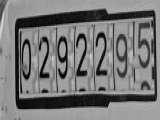
\includegraphics[width=0.9\linewidth]{assets/apresentacao/esp32_22.jpg}\\[2pt]
    {\tiny Hidrômetro visto pela câmera do nó (160$\times$120)}
  \end{columns}
\end{frame}

\begin{frame}{Introdução - Contexto}
  \centering
  \begin{tikzpicture}[
      font=\small,
      caixa/.style={draw, rounded corners=3pt, align=center, minimum height=1.1cm, text width=3.1cm, fill=white},
      seta/.style={-{Stealth[length=2mm]}, thick}]
    \node[caixa] (cam) {\textbf{Nó sensor}\\ESP32-CAM};
    \node[caixa, draw=corBorda, line width=1pt, above right=0.2cm and 1.6cm of cam] (b) {\color{corBorda}\textbf{Borda}\\OCR no nó\\envia \textbf{9 bytes}};
    \node[caixa, draw=corNuvem, line width=1pt, below right=0.2cm and 1.6cm of cam] (n) {\color{corNuvem}\textbf{Nuvem}\\envia a \textbf{imagem}\\OCR no servidor};
    \node[caixa, right=1.6cm of $(b)!0.5!(n)$] (s) {\textbf{Servidor}\\leitura registrada};
    \draw[seta] (cam) -- (b); \draw[seta] (cam) -- (n);
    \draw[seta] (b) -- (s); \draw[seta] (n) -- (s);
  \end{tikzpicture}

  \vspace{0.5cm}
  {\small Qual escolha gasta menos energia, responde mais rápido e erra menos?}
\end{frame}

% ===============================================================
\section{Objetivos e método}
% ===============================================================

\begin{frame}{Objetivos}
  \begin{block}{Objetivo geral}
    Comparar a viabilidade técnica, a acurácia e o consumo energético do OCR feito
    \textbf{no ESP32-CAM} (borda) e \textbf{em um servidor} (nuvem), usando LoRaWAN como meio
    de transmissão.
  \end{block}
  \vspace{0.15cm}
  {\small\bfseries\color{senacblue}Objetivos específicos}
  \vspace{0.1cm}
  \small
  \renewcommand{\arraystretch}{1.3}
  \begin{tabular}{@{}r >{\raggedright\arraybackslash}p{10.6cm} l@{}}
    \textbf{\color{senacorange}1} & Implementar os dois fluxos: OCR no nó e envio da imagem para o servidor. \\
    \textbf{\color{senacorange}2} & Configurar a rede LoRaWAN buscando o menor consumo possível.  \\
    \textbf{\color{senacorange}3} & Avaliar os fluxos em acurácia (\%), latência (s), energia por leitura (mAh) e volume de dados (bytes). \\
  \end{tabular}
  \vspace{0.1cm}
  {\scriptsize\color{black!60}}
\end{frame}

\begin{frame}{Hipóteses}
  \centering
  \vspace*{-0.4cm}
  \begin{tikzpicture}[
      cartao/.style={draw=senacblue, rounded corners=4pt, fill=senacblue!5,
                     text width=4.1cm, minimum height=3.9cm, align=flush left, inner sep=6pt,
                     anchor=north},
      cab/.style={font=\Large\bfseries, text=senacorange}]
    \node[cartao] (h1) at (0,0) {%
      {\large\bfseries\color{senacorange}H1}\\[2pt]
      {\scriptsize\bfseries A quantização em INT8 do modelo da borda reduz a acurácia em relação ao modelo em float32}\\[5pt]};
    \node[cartao] (h2) at (4.85,0) {%
      {\large\bfseries\color{senacorange}H2}\\[2pt]
      {\scriptsize\bfseries O processamento local tem custo computacional maior no dispositivo final}\\[5pt]};
    \node[cartao] (h3) at (9.7,0) {%
      {\large\bfseries\color{senacorange}H3}\\[2pt]
      {\scriptsize\bfseries A nuvem tem autonomia energética inferior durante a transmissão}\\[5pt]};
  \end{tikzpicture}
\end{frame}

\begin{frame}{Como cada hipótese é testada}
  \centering
  \footnotesize
  \renewcommand{\arraystretch}{1.35}
  \begin{tabular}{@{}l >{\raggedright\arraybackslash}p{3.4cm} >{\raggedright\arraybackslash}p{4.4cm} >{\raggedright\arraybackslash}p{3.0cm}@{}}
    \toprule
    & \textbf{Métrica} & \textbf{Como medimos} & \textbf{Teste} \\
    \midrule
    \textbf{\color{senacorange}H1} & Acurácia por dígito e leitura exata
      & 7.378 dígitos de teste, float32 × INT8 & McNemar (pareado) \\
    \textbf{\color{senacorange}H2} & Tempo de processamento e memória no nó
      & tempo até a leitura (ou imagem) pronta no nó; uso da PSRAM & comparação direta \\
    \textbf{\color{senacorange}H3} & Carga por leitura (mAh) e autonomia
      & INA219 a 100 amostras/s em 30 ciclos por fluxo & razão entre fluxos e modelo de autonomia \\
    \bottomrule
  \end{tabular}

  \vspace{0.4cm}
\end{frame}

\begin{frame}{Método}
  \centering
  \begin{tikzpicture}[
      font=\footnotesize,
      etapa/.style={draw=senacblue, rounded corners=3pt, fill=senacblue!8, align=center,
                    minimum height=1.3cm, text width=2.05cm},
      seta/.style={-{Stealth[length=2mm]}, thick, senacblue}]
    \node[etapa] (a) {\textbf{1}\\Implementar os dois fluxos};
    \node[etapa, right=0.35cm of a] (b) {\textbf{2}\\Treinar e quantizar o OCR};
    \node[etapa, right=0.35cm of b] (c) {\textbf{3}\\Rodar em bancada (30 leituras)};
    \node[etapa, right=0.35cm of c] (d) {\textbf{4}\\Medir corrente, tempo e pacotes};
    \node[etapa, right=0.35cm of d] (e) {\textbf{5}\\Testes estatísticos};
    \draw[seta] (a) -- (b); \draw[seta] (b) -- (c); \draw[seta] (c) -- (d); \draw[seta] (d) -- (e);
  \end{tikzpicture}

  \vspace{0.6cm}
  {\small Pesquisa experimental e quantitativa \quad·\quad mesmo hardware, mesma imagem, mesmo modelo}

  \vspace{0.2cm}
  {\scriptsize\color{black!60} Dados brutos e \textit{scripts} versionados no repositório do projeto}
\end{frame}

% ===============================================================
\section{Desenvolvimento}
% ===============================================================
\begin{frame}{Hardware}
  \begin{columns}[c]
    \column{0.58\textwidth}
    \centering
    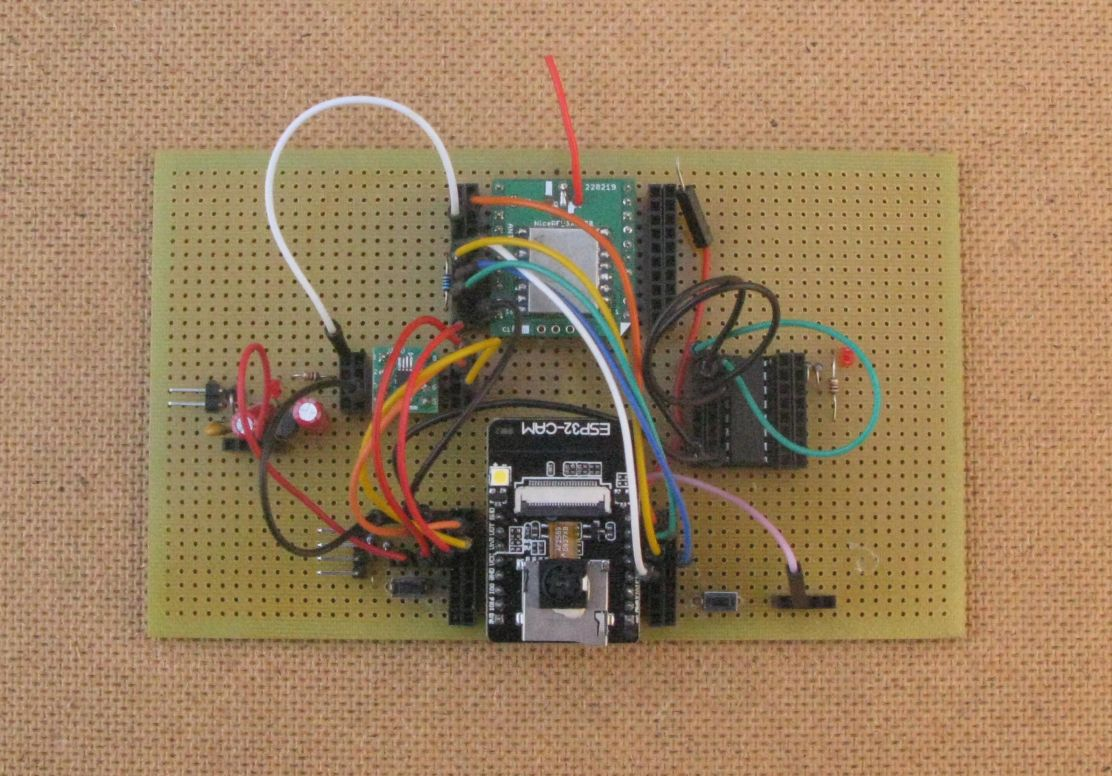
\includegraphics[width=\linewidth]{sections/imagens/ESP32CAM_LoRa.jpg}\\[1pt]
    {\tiny Nó sensor: ESP32-CAM + Radioenge RD49C}
    \column{0.4\textwidth}
    \begin{itemize}\small
      \item \textbf{ESP32-CAM}: câmera e OCR
      \item \textbf{RD49C}: rádio LoRaWAN por comandos AT
      \item \textbf{LoRa32}: receptor no canal 915,9~MHz
      \item \textbf{INA219}: corrente a 100~Hz
    \end{itemize}
  \end{columns}
\end{frame}

\begin{frame}[fragile]{Arquitetura}
  \centering
  \begin{tikzpicture}[
      font=\scriptsize,
      bloco/.style={draw, rounded corners=2pt, align=center, fill=white, minimum height=0.9cm, text width=#1},
      bloco/.default=2.4cm,
      seta/.style={-{Stealth[length=1.8mm]}, thick}]
    \node[bloco=1.8cm] (h) {Hidrômetro};
    \node[bloco, right=0.5cm of h] (c) {\textbf{ESP32-CAM}\\foto 160$\times$120};
    \node[bloco=2.6cm, draw=corBorda, line width=1pt, above right=0.15cm and 0.6cm of c] (b) {\color{corBorda}\textbf{Borda}: OCR INT8\\1 pacote de 9~B};
    \node[bloco=2.6cm, draw=corNuvem, line width=1pt, below right=0.15cm and 0.6cm of c] (n) {\color{corNuvem}\textbf{Nuvem}: JPEG $\approx$4~KB\\24 blocos de 175~B};
    \node[bloco=2.2cm, right=3.6cm of c] (r) {\textbf{RD49C}\\AU915 · DR6};
    \node[bloco=2.0cm, right=0.5cm of r] (p) {\textbf{Servidor}\\remonta e lê};
    \draw[seta] (h) -- (c); \draw[seta] (c) -- (b.west); \draw[seta] (c) -- (n.west);
    \draw[seta] (b.east) -- (r); \draw[seta] (n.east) -- (r); \draw[seta] (r) -- (p);
  \end{tikzpicture}

  \vspace{0.5cm}
  \begin{columns}[t]
    \column{0.3\textwidth}\centering{\footnotesize\textbf{SF8 / 500~kHz}\\\scriptsize item 10.3 do Ato ANATEL 14.448}
    \column{0.3\textwidth}\centering{\footnotesize\textbf{7~s entre blocos}\\\scriptsize espera do rádio}
    \column{0.3\textwidth}\centering{\footnotesize\textbf{AES + MIC}\\\scriptsize ativação ABP}
  \end{columns}
\end{frame}

\begin{frame}{OCR em duas etapas}
  \centering
  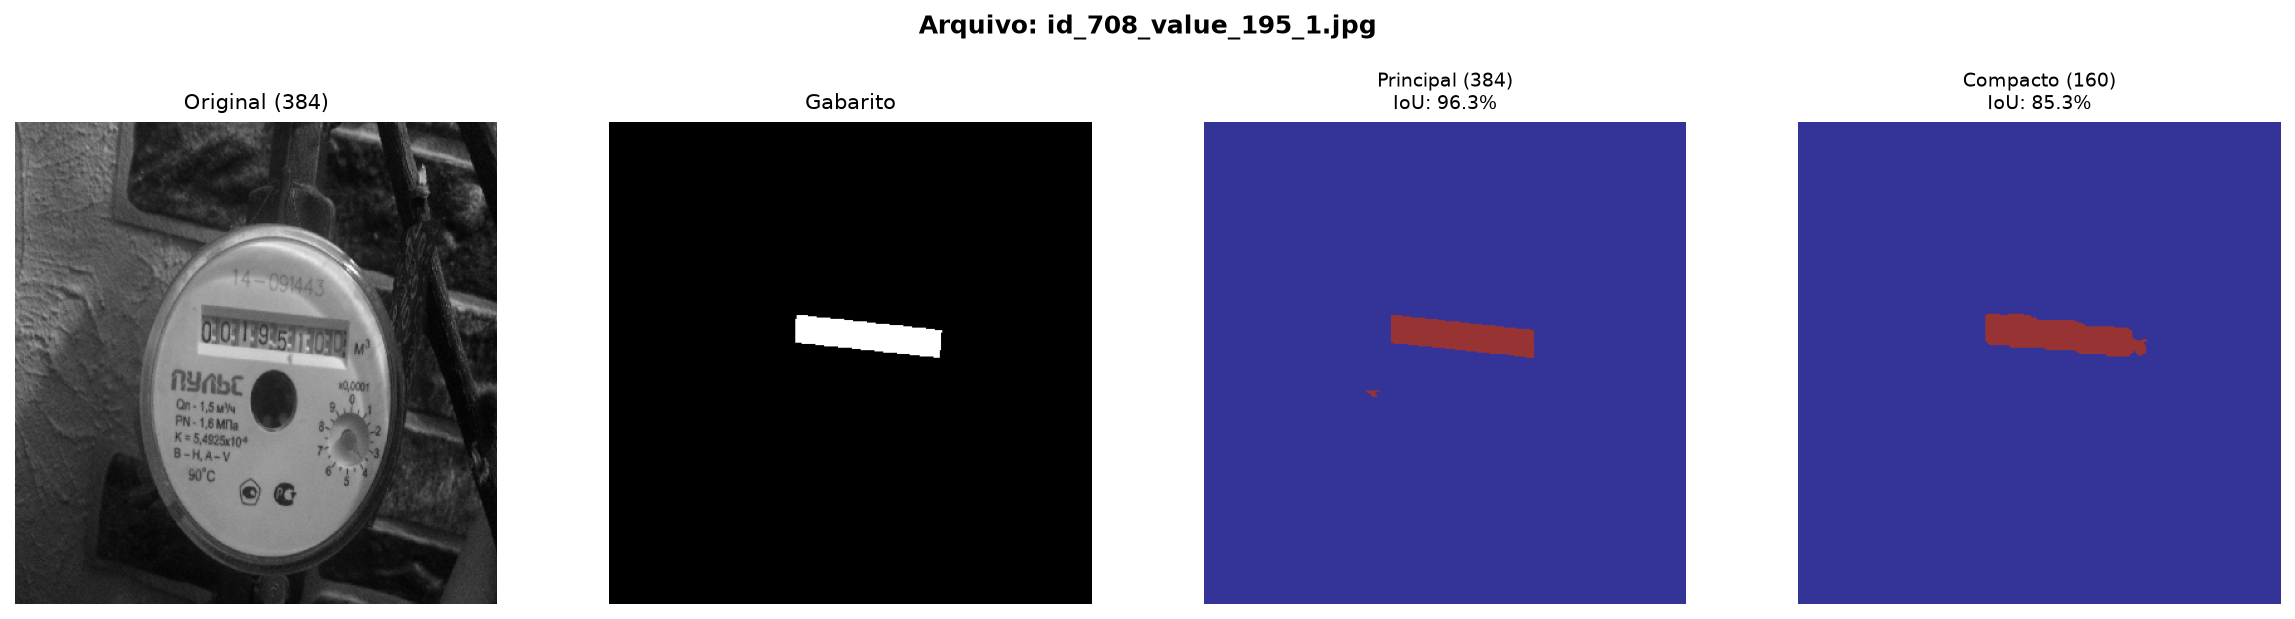
\includegraphics[width=0.95\textwidth]{sections/imagens/testeUNet_1.png}\\[2pt]
  {\tiny Segmentação do visor (U-Net): original, gabarito e previsões}

  \vspace{0.3cm}
  \begin{columns}[t]
    \column{0.3\textwidth}\centering
    {\Large\bfseries\color{senacblue}1}\\{\scriptsize Localiza o visor}
    \column{0.3\textwidth}\centering
    {\Large\bfseries\color{senacblue}2}\\{\scriptsize Fatia em dígitos}
    \column{0.3\textwidth}\centering
    {\Large\bfseries\color{senacblue}3}\\{\scriptsize CNN 28$\times$28 classifica 0--9}
  \end{columns}
\end{frame}

\begin{frame}{Treinamento}
  \centering
  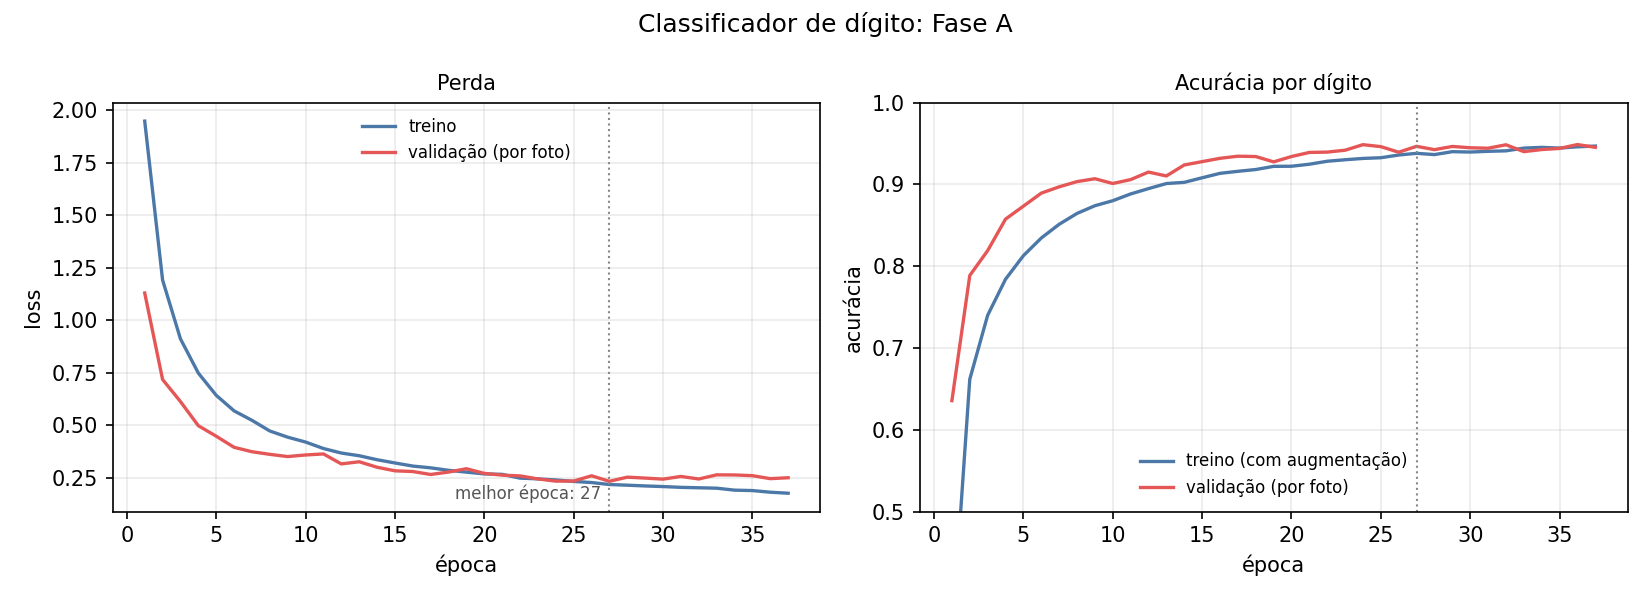
\includegraphics[width=0.8\textwidth]{sections/imagens/ocr_treino_classificador.png}\\[2pt]
  {\tiny Curvas de treino do classificador de dígitos}

  \vspace{0.3cm}
  \begin{columns}[t]
    \column{0.3\textwidth}\bignum[senacblue]{72 mil}{parâmetros na CNN}
    \column{0.3\textwidth}\bignum[senacblue]{49 mil}{recortes de dígitos no treino}
    \column{0.3\textwidth}\bignum[senacblue]{INT8}{quantização pós-treino}
  \end{columns}
\end{frame}

\begin{frame}{Leitura no nó}
  \begin{columns}[c]
    \column{0.42\textwidth}
    \centering
    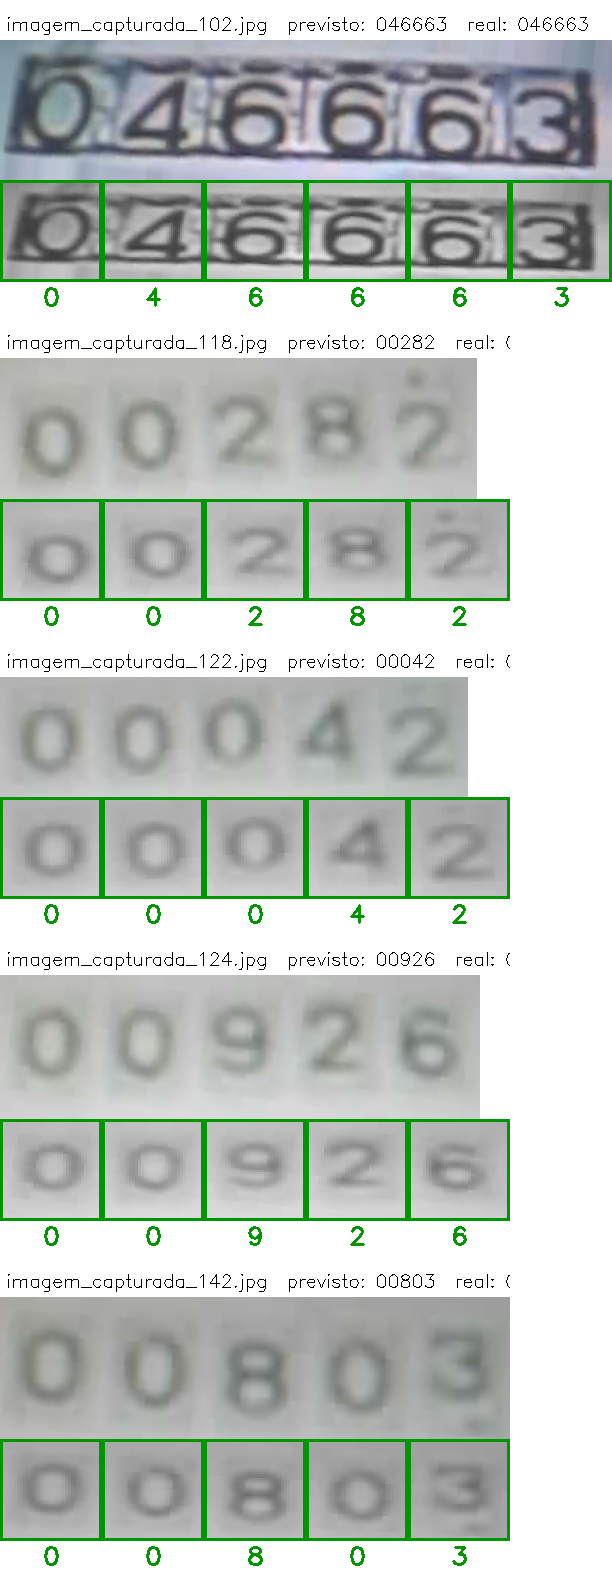
\includegraphics[width=0.9\linewidth,trim=0 1265 0 0,clip]{sections/imagens/ocr_leitura_caixa_manual.png}\\[2pt]
    {\tiny Visor recortado, dígitos e leitura prevista}
    \column{0.55\textwidth}
    \begin{itemize}\small
      \item Câmera fixa: a janela dos dígitos é \textbf{calibrada uma vez}.
      \item Corta, fatia e classifica cada dígito.
      \item Roda no ESP32-CAM com TFLite Micro.
      \item Resultado: uma leitura de \textbf{9 bytes}.
    \end{itemize}
  \end{columns}
\end{frame}

\begin{frame}{Bancada de testes}
  \begin{columns}[c]
    \column{0.42\textwidth}
    \centering
    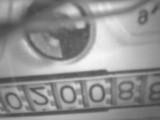
\includegraphics[width=0.85\linewidth]{assets/apresentacao/bancada_quadro.jpg}\\[2pt]
    {\tiny Quadro capturado pelo nó na bancada}
    \column{0.56\textwidth}
    \centering
    \begin{tikzpicture}[
        font=\scriptsize,
        bloco/.style={draw, rounded corners=2pt, align=center, fill=white, minimum height=0.8cm, text width=1.9cm},
        seta/.style={-{Stealth[length=1.6mm]}, thick}]
      \node[bloco] (mb) {Fonte USB 5~V};
      \node[bloco, right=0.5cm of mb] (ina) {\textbf{INA219}\\\textit{shunt} 0,1~$\Omega$};
      \node[bloco, below=0.5cm of ina] (no) {\textbf{Nó sensor}\\câmera + rádio};
      \node[bloco, below=0.5cm of mb] (uno) {Arduino\\100 amostras/s};
      \draw[seta] (mb) -- (ina); \draw[seta] (ina) -- (no); \draw[seta] (ina) -- (uno);
    \end{tikzpicture}

    \vspace{0.3cm}
    {\footnotesize 30 ciclos por fluxo · leitura a cada ciclo}
  \end{columns}
\end{frame}

% ===============================================================
\section{Resultados parciais}
% ===============================================================
{
\setbeamercolor{background canvas}{bg=senacblue!6}
\begin{frame}{Resultados em números}
  \vspace{0.2cm}
  \begin{columns}[t]
    \column{0.32\textwidth}\bignum[corBorda]{10$\times$}{menor latência na borda\\(18,8~s contra 189~s)}
    \column{0.32\textwidth}\bignum[corBorda]{5,6$\times$}{menos energia por leitura\\(0,82 contra 4,64~mAh)}
    \column{0.32\textwidth}\bignum[senacblue]{99,6\%}{concordância float × INT8\\nos mesmos dígitos}
  \end{columns}
  \vspace{0.6cm}
  \begin{columns}[t]
    \column{0.32\textwidth}\bignum[corBorda]{450$\times$}{menos dados no ar\\(9~B contra $\approx$4~KB)}
    \column{0.32\textwidth}\bignum[senacblue]{97,7\%}{dígitos corretos em\\conjunto independente}
    \column{0.32\textwidth}\bignum[corFalha]{56\%}{dígitos corretos em\\hidrômetros reais (21 fotos)}
  \end{columns}
\end{frame}
}

\begin{frame}{H1 --- Quantização INT8}
  \begin{columns}[c]
    \column{0.55\textwidth}
    \centering
    \begin{tikzpicture}
      \begin{axis}[estiloSlides, ybar, width=\linewidth, height=5.2cm,
          bar width=1.1cm, ymin=90, ymax=97, enlarge x limits=0.6,
          symbolic x coords={Float32,INT8}, xtick=data,
          ylabel={Acurácia por dígito (\%)},
          nodes near coords, nodes near coords style={font=\footnotesize\bfseries},
          point meta=explicit symbolic]
        \addplot[fill=senacblue!70, draw=none] coordinates {(Float32,95.46) [95,46] (INT8,95.38) [95,38]};
      \end{axis}
    \end{tikzpicture}
    \column{0.42\textwidth}
    \begin{itemize}\small
      \item 7.378 dígitos de teste
      \item Diferença: \textbf{6 dígitos}
      \item McNemar: $p = 0{,}29$
    \end{itemize}
    \vspace{0.2cm}
    \etiqueta{senacorange}{CONFIRMADA NA DIREÇÃO}\\[2pt]
    {\scriptsize mas a perda é desprezível}
  \end{columns}
\end{frame}

\begin{frame}{H2 --- Custo computacional no nó}
  \begin{columns}[c]
    \column{0.55\textwidth}
    \centering
    \begin{tikzpicture}
      \begin{axis}[estiloSlides, xbar, width=\linewidth, height=4.2cm,
          bar width=0.6cm, xmin=0, xmax=23, enlarge y limits=0.5,
          symbolic y coords={Nuvem,Borda}, ytick={Nuvem,Borda},
          xlabel={Tempo até o dado pronto no nó (s)},
          nodes near coords, nodes near coords style={font=\footnotesize\bfseries, anchor=west},
          point meta=explicit symbolic]
        \addplot[fill=corNuvem, draw=none, bar shift=0pt] coordinates {(0.70,Nuvem) [0,7~s]};
        \addplot[fill=corBorda, draw=none, bar shift=0pt] coordinates {(18.20,Borda) [18,2~s]};
      \end{axis}
    \end{tikzpicture}\\[2pt]
    {\tiny Borda: captura + OCR · Nuvem: captura da imagem}
    \column{0.42\textwidth}
    \centering
    {\fontsize{22}{24}\selectfont\bfseries\color{corBorda}1,65~MB\par}
    {\scriptsize\color{black!70}PSRAM usada pelo OCR na borda\par}
    \vspace{0.2cm}
    {\fontsize{22}{24}\selectfont\bfseries\color{corBorda}114~mA\par}
    {\scriptsize\color{black!70}corrente durante a inferência\par}
    \vspace{0.3cm}
    {\scriptsize Mesmo OCR: 17,8~s no ESP32 e 6,25~ms no servidor}\\[4pt]
    \etiqueta{corOk}{CONFIRMADA}
  \end{columns}
\end{frame}

\begin{frame}{Rede --- Latência}
  \begin{columns}[c]
    \column{0.6\textwidth}
    \centering
    \begin{tikzpicture}
      \begin{axis}[estiloSlides, xbar, width=\linewidth, height=4.2cm,
          bar width=0.6cm, xmin=0, xmax=240, enlarge y limits=0.5,
          symbolic y coords={Borda,Nuvem}, ytick={Borda,Nuvem},
          xlabel={Latência mediana por leitura (s)},
          nodes near coords, nodes near coords style={font=\footnotesize\bfseries, anchor=west},
          point meta=explicit symbolic]
        \addplot[fill=corBorda, draw=none, bar shift=0pt] coordinates {(18.84,Borda) [18,8~s]};
        \addplot[fill=corNuvem, draw=none, bar shift=0pt] coordinates {(189.1,Nuvem) [189~s]};
      \end{axis}
    \end{tikzpicture}
    \column{0.37\textwidth}
    \begin{itemize}\small
      \item Nuvem: 24 blocos com 7~s de intervalo
      \item Borda: inferência $\approx$18~s + 1 pacote
    \end{itemize}
    \vspace{0.2cm}
    {\scriptsize Borda entrega a leitura \textbf{10$\times$ mais rápido}}
  \end{columns}
\end{frame}

\begin{frame}{Rede --- Entrega}
  \begin{columns}[c]
    \column{0.6\textwidth}
    \centering
    \begin{tikzpicture}
      \begin{axis}[estiloSlides, ybar, width=\linewidth, height=5.2cm,
          bar width=0.7cm, ymin=0, ymax=110, enlarge x limits=0.45,
          symbolic x coords={Pacotes,Leituras completas}, xtick=data,
          ylabel={Taxa de entrega (\%)},
          legend style={at={(0.5,1.02)}, anchor=south, legend columns=2},
          nodes near coords, nodes near coords style={font=\scriptsize\bfseries},
          point meta=explicit symbolic]
        \addplot[fill=corNuvem, draw=none] coordinates {(Pacotes,98.0) [98,0] (Leituras completas,66.7) [66,7]};
        \addplot[fill=corBorda, draw=none] coordinates {(Pacotes,79.4) [79,4] (Leituras completas,79.4) [79,4]};
        \legend{Nuvem, Borda}
      \end{axis}
    \end{tikzpicture}
    \column{0.37\textwidth}
    \begin{itemize}\small
      \item Nuvem perde \textbf{1 bloco} e perde a leitura
      \item Por leitura: Fisher $p = 0{,}27$
    \end{itemize}
    \vspace{0.2cm}
    {\scriptsize Por leitura, a diferença \textbf{não é significativa}}
  \end{columns}
\end{frame}

\begin{frame}{H3 --- Corrente em um ciclo}
  \centering
  \begin{tikzpicture}
    \begin{groupplot}[estiloSlides,
        group style={group size=1 by 2, vertical sep=1.3cm},
        width=0.95\textwidth, height=3.1cm,
        xmin=0, xmax=225, ymin=0, ymax=250, ytick={0,100,200},
        ylabel={mA}]
      \nextgroupplot[title={\color{corNuvem}Nuvem: 4,65~mAh por leitura}]
      \addplot[color=corNuvem, line width=0.35pt] table {sections/dados/corrente_ciclo_nuvem.dat};
      \nextgroupplot[title={\color{corBorda}Borda: 0,82~mAh por leitura}, xlabel={Tempo desde o despertar (s)}]
      \addplot[color=corBorda, line width=0.35pt] table {sections/dados/corrente_ciclo_borda.dat};
    \end{groupplot}
  \end{tikzpicture}
\end{frame}

\begin{frame}{H3 --- Energia e autonomia}
  \begin{columns}[c]
    \column{0.5\textwidth}
    \centering
    \begin{tikzpicture}
      \begin{axis}[estiloSlides, ybar, width=\linewidth, height=5cm,
          bar width=1cm, ymin=0, ymax=5.5, enlarge x limits=0.6,
          symbolic x coords={Nuvem,Borda}, xtick={Nuvem,Borda},
          ylabel={Carga por leitura (mAh)},
          nodes near coords, nodes near coords style={font=\footnotesize\bfseries},
          point meta=explicit symbolic]
        \addplot[fill=corNuvem, draw=none, bar shift=0pt] coordinates {(Nuvem,4.64) [4,64]};
        \addplot[fill=corBorda, draw=none, bar shift=0pt] coordinates {(Borda,0.824) [0,82]};
      \end{axis}
    \end{tikzpicture}
    \column{0.47\textwidth}
    \begin{itemize}\small
      \item Nuvem acorda \textbf{10$\times$ mais tempo}
      \item Repouso de \textbf{24~mA} limita a autonomia
      \item Ganho de autonomia: \textbf{1,0 a 7,0$\times$}, conforme o intervalo
    \end{itemize}
    \vspace{0.2cm}
    \etiqueta{corOk}{CONFIRMADA}
  \end{columns}
\end{frame}

\begin{frame}{Comparação dos fluxos}
  \centering
  \small
  \begin{tabular}{lrr}
    \toprule
    & \textbf{\color{corNuvem}Nuvem} & \textbf{\color{corBorda}Borda} \\
    \midrule
    Dados por leitura        & $\approx$4~KB (24 blocos) & 9~B (1 pacote) \\
    Latência mediana         & 189~s     & 18,8~s \\
    Carga por leitura        & 4,64~mAh  & 0,82~mAh \\
    Pacotes entregues        & 98,0\%    & 79,4\% \\
    Leituras completas       & 66,7\%    & 79,4\% \\
    Inferência               & 6,25~ms (PC) & $\approx$18~s (ESP32) \\
    Atualizar o modelo       & só no servidor & regravar o nó \\
    \bottomrule
  \end{tabular}

  \vspace{0.3cm}
  {\scriptsize\color{black!60} Mesmo modelo INT8 nos dois fluxos}
\end{frame}

\begin{frame}{Hidrômetros reais: onde ainda falha}
  \begin{columns}[c]
    \column{0.55\textwidth}
    \centering
    \begin{tabular}{@{}c@{\hspace{3pt}}c@{}}
      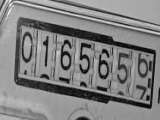
\includegraphics[width=0.44\linewidth]{assets/apresentacao/esp32_04.jpg} &
      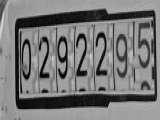
\includegraphics[width=0.44\linewidth]{assets/apresentacao/esp32_22.jpg} \\
      \multicolumn{2}{c}{\tiny\color{corOk}\textbf{Fundo claro e frontal: acerta}} \\[3pt]
      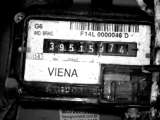
\includegraphics[width=0.44\linewidth]{assets/apresentacao/esp32_02.jpg} &
      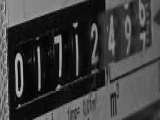
\includegraphics[width=0.44\linewidth]{assets/apresentacao/esp32_21.jpg} \\
      \multicolumn{2}{c}{\tiny\color{corFalha}\textbf{Fundo escuro ou inclinado: erra}}
    \end{tabular}
    \column{0.43\textwidth}
    \centering
    \footnotesize
    \begin{tabular}{lr}
      \toprule
      \textbf{Grupo (21 fotos)} & \textbf{Dígitos} \\
      \midrule
      Fundo claro, frontal  & 90\% \\
      Fundo escuro          & 12\% \\
      \quad invertido       & 43\% \\
      \bottomrule
    \end{tabular}

    \vspace{0.3cm}
    {\scriptsize Fundo escuro é só \textbf{0,9\%} do treino}
  \end{columns}
\end{frame}

\begin{frame}{Síntese das hipóteses}
  \centering
  \footnotesize
  \begin{tabular}{llc}
    \toprule
    \textbf{Hipótese} & \textbf{Evidência} & \textbf{Situação} \\
    \midrule
    H1 --- INT8 reduz acurácia     & 95,46\% $\rightarrow$ 95,38\%, $p=0{,}29$ & \etiqueta{senacorange}{DESPREZÍVEL} \\[2pt]
    H2 --- maior custo no nó (borda) & 18,2 contra 0,7~s; 1,65~MB  & \etiqueta{corOk}{CONFIRMADA} \\[2pt]
    H3 --- nuvem com menor autonomia & 4,64 contra 0,82~mAh                   & \etiqueta{corOk}{CONFIRMADA} \\
    \bottomrule
  \end{tabular}

  \vspace{0.4cm}
  {\scriptsize\color{black!60} Rede (complementar): borda 10$\times$ mais rápida; entrega por leitura
  79\% contra 67\%, sem significância ($p=0{,}27$)}
\end{frame}

% ===============================================================
\section{Andamento}
% ===============================================================
\begin{frame}{Andamento do trabalho}
  \begin{columns}[t]
    \column{0.32\textwidth}
    {\small\bfseries\color{corOk}Concluído}
    \begin{itemize}\scriptsize
      \item Dois fluxos funcionando
      \item Treino e quantização do OCR
      \item Medições de bancada
      \item Testes estatísticos
      \item Capítulo de desenvolvimento e resultados
    \end{itemize}
    \column{0.32\textwidth}
    {\small\bfseries\color{senacorange}Em andamento}
    \begin{itemize}\scriptsize
      \item Conclusão
      \item Resumo e \textit{abstract}
      \item Revisão da H1 e da metodologia
      \item Ajustes no referencial teórico
    \end{itemize}
    \column{0.32\textwidth}
    {\small\bfseries\color{senacblue}Próximos passos}
    \begin{itemize}\scriptsize
      \item Suspender o rádio no repouso
      \item Mais fotos de fundo escuro no treino
      \item Medir a borda com janela fixa no nó
      \item Ensaiar a apresentação final
    \end{itemize}
  \end{columns}

  \vspace{0.4cm}
  \centering
  \begin{tikzpicture}
    \fill[black!10, rounded corners=2pt] (0,0) rectangle (10.5,0.3);
    \fill[corOk, rounded corners=2pt] (0,0) rectangle (8.4,0.3);
    \node[font=\scriptsize\bfseries, anchor=west] at (10.6,0.15) {$\approx$80\% (estimativa)};
  \end{tikzpicture}
\end{frame}

\begin{frame}{Conclusão parcial}
  \begin{itemize}
    \item \textbf{Borda}: mais rápida e mais econômica.
    \item \textbf{Nuvem}: mais fácil de manter e atualizar.
    \item Quantização INT8 \textbf{não} é o gargalo da acurácia.
    \item O gargalo é a \textbf{captura}: ângulo, luz e fundo do mostrador.
  \end{itemize}
\end{frame}

% ---------------------------------------------------------------
% ENCERRAMENTO
% ---------------------------------------------------------------
\begin{frame}[plain]
  \centering
  \vspace{1cm}
  \logosenacgrande

  \vspace{0.8cm}
  {\Large\bfseries\color{senacblue}Obrigado!\par}
  \vspace{0.3cm}
  {\normalsize Perguntas e sugestões?\par}
\end{frame}

% ---------------------------------------------------------------
% APÊNDICE
% ---------------------------------------------------------------
\appendix

\begin{frame}{Apoio --- Autonomia (leitura a cada 1~h)}
  \centering
  \begin{tikzpicture}[declare function={autonomia(\i,\a,\r,\T) = 83.3333*\T/(\i*\a + \r*(\T - \a));}]
    \begin{axis}[estiloSlides, width=0.8\textwidth, height=5.4cm,
        xmode=log, ymode=log, xmin=0.01, xmax=30, ymin=1, ymax=3000,
        xtick={0.01,0.1,1,10}, xticklabels={{0,01},{0,1},1,10},
        ytick={1,10,100,1000}, yticklabels={1,10,100,{1.000}},
        xlabel={Corrente em repouso (mA)}, ylabel={Autonomia (dias)},
        legend pos=south west]
      \addplot[color=corNuvem, line width=1pt, domain=-2:1.4771, samples=60]
        ({10^x}, {autonomia(84.5,189.9,10^x,3600)});
      \addlegendentry{Nuvem}
      \addplot[color=corBorda, line width=1pt, densely dashed, domain=-2:1.4771, samples=60]
        ({10^x}, {autonomia(114.4,19.45,10^x,3600)});
      \addlegendentry{Borda}
      \draw[color=black!55, line width=0.5pt] (axis cs:24,1) -- (axis cs:24,3000)
        node[pos=0.9, anchor=east, font=\tiny] {medido: 24~mA};
    \end{axis}
  \end{tikzpicture}

  {\tiny Bateria hipotética de 2.000~mAh}
\end{frame}

\begin{frame}{Apoio --- Conjunto físico completo}
  \centering
  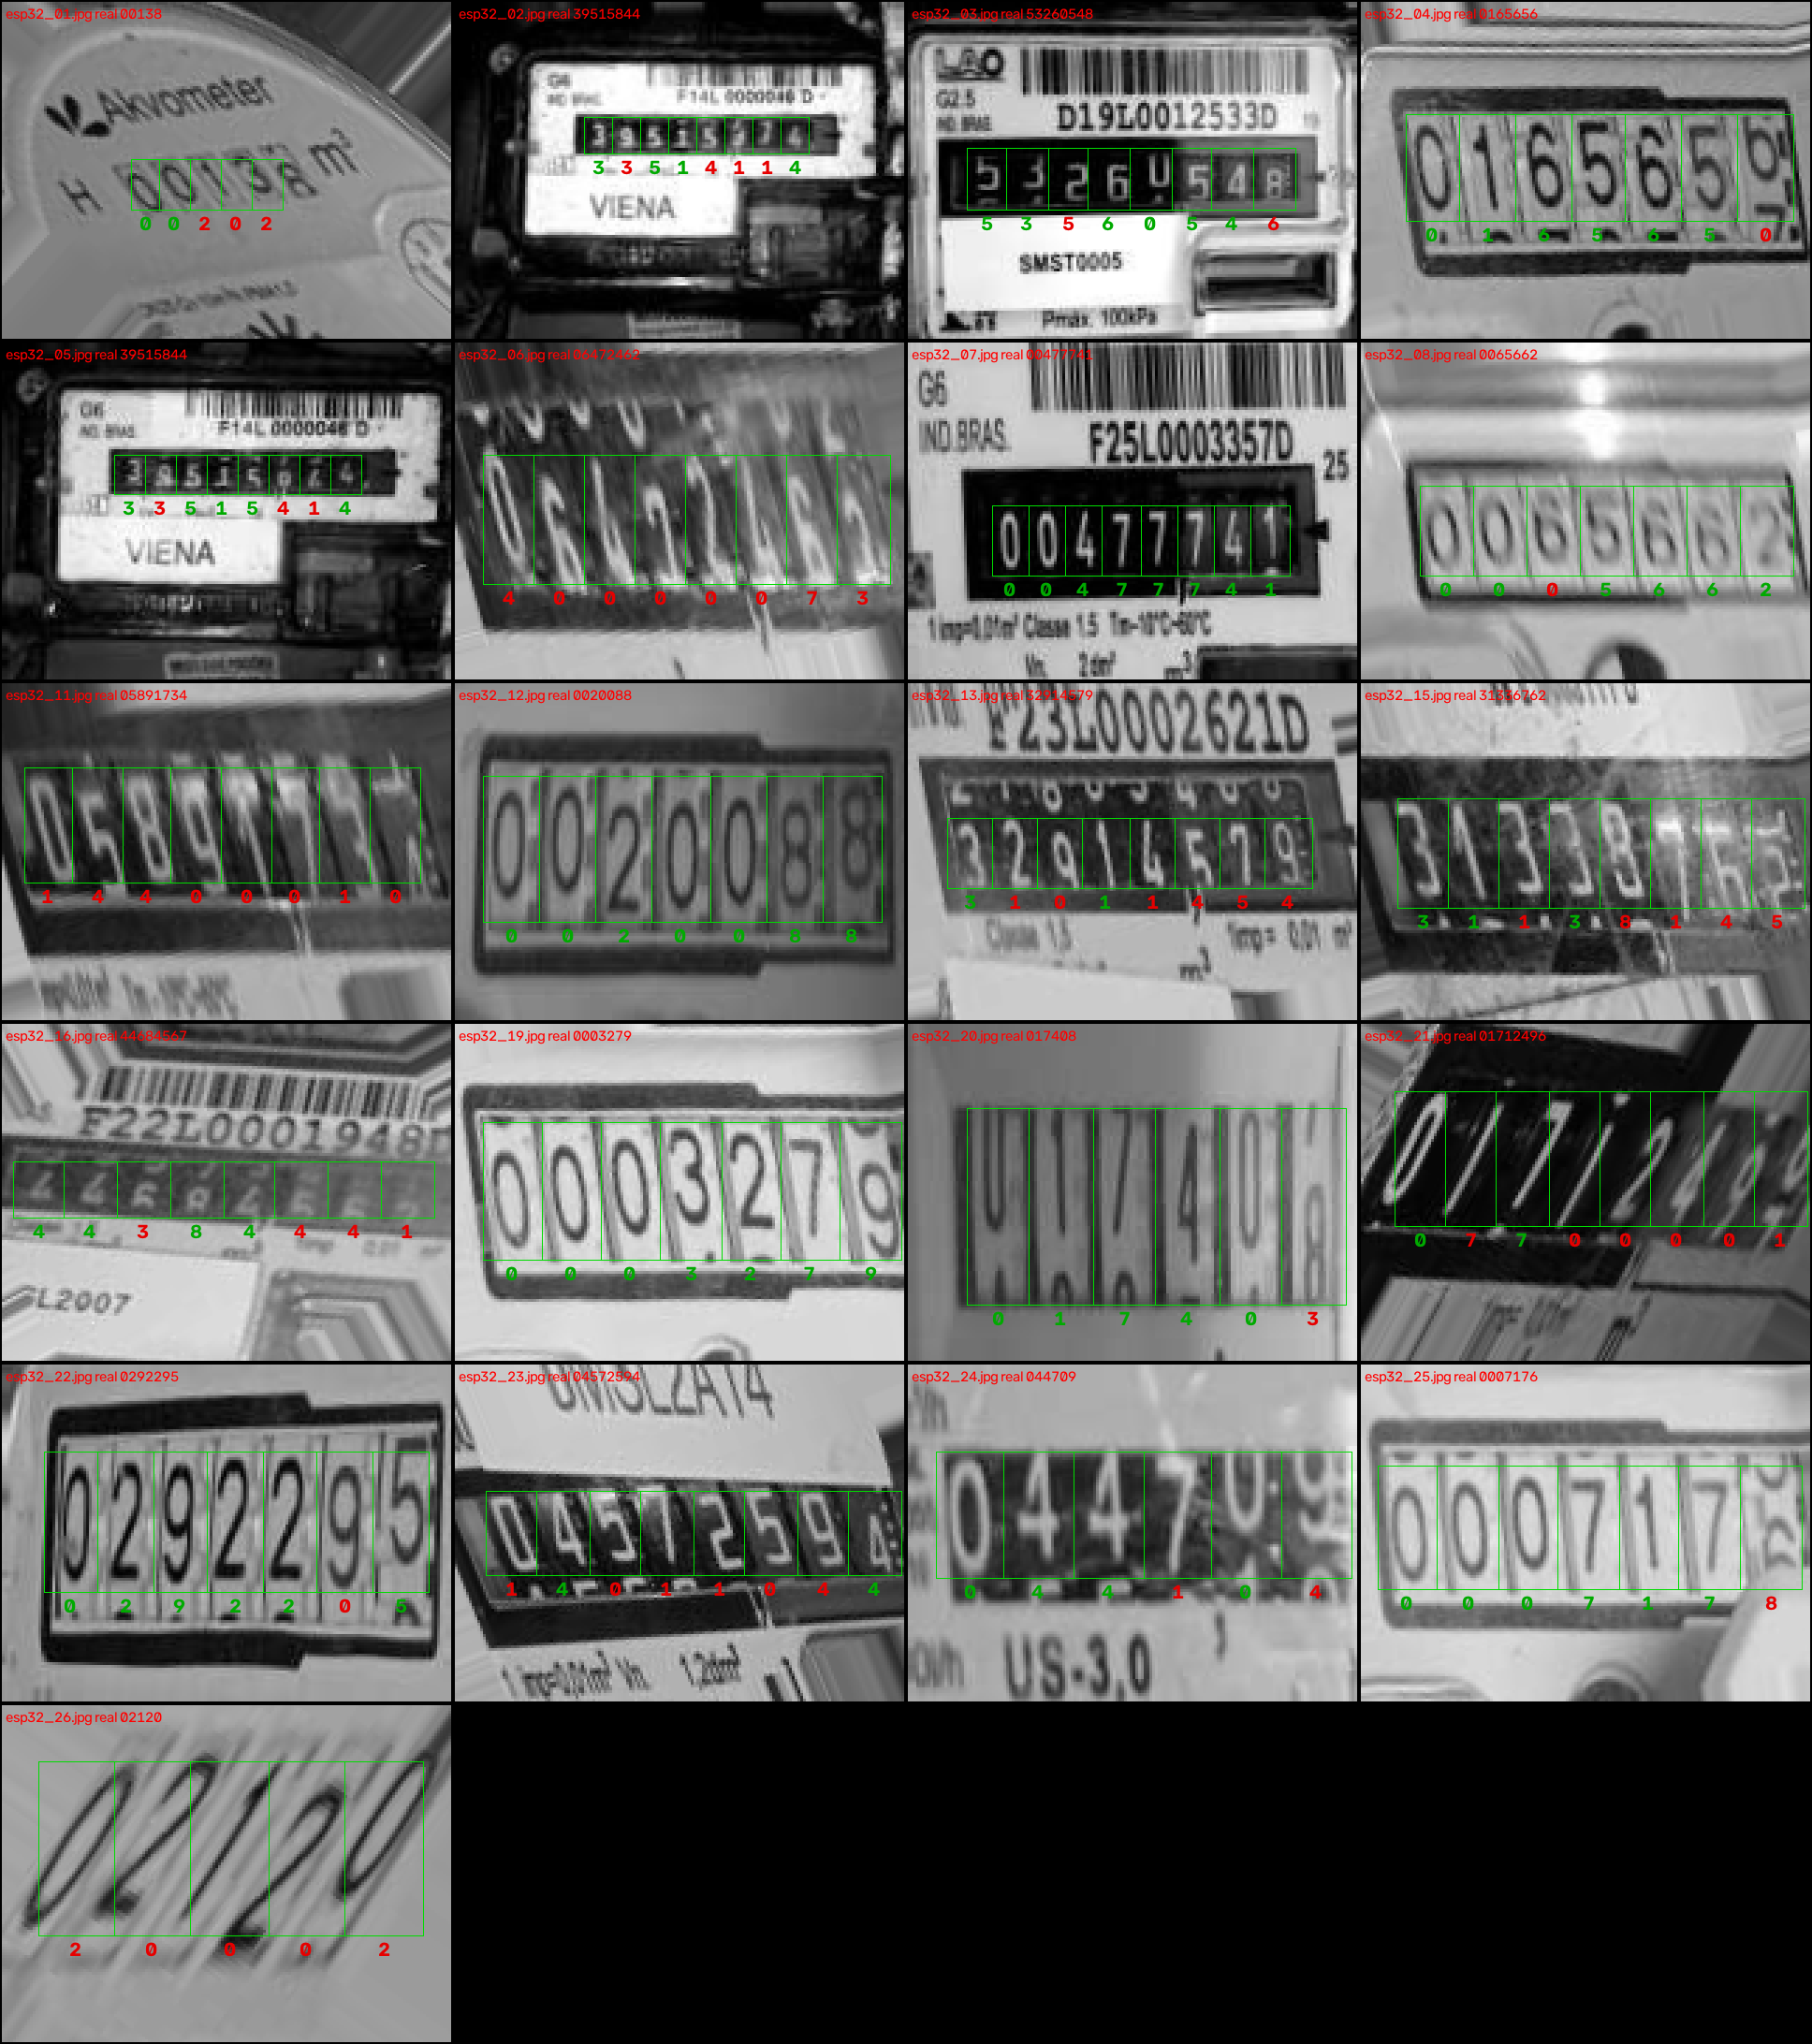
\includegraphics[height=0.75\textheight]{assets/apresentacao/conjunto_fisico.png}\\
  {\tiny Verde: dígito correto · vermelho: dígito errado}
\end{frame}

\end{document}
